\documentclass{ximera}

%\usepackage{todonotes}

\newcommand{\todo}{}

\usepackage{esint} % for \oiint
\ifxake%%https://math.meta.stackexchange.com/questions/9973/how-do-you-render-a-closed-surface-double-integral
\renewcommand{\oiint}{{\large\bigcirc}\kern-1.56em\iint}
\fi


\graphicspath{
  {./}
  {ximeraTutorial/}
  {basicPhilosophy/}
  {functionsOfSeveralVariables/}
  {normalVectors/}
  {lagrangeMultipliers/}
  {vectorFields/}
  {greensTheorem/}
  {shapeOfThingsToCome/}
  {dotProducts/}
  {partialDerivativesAndTheGradientVector/}
  {../productAndQuotientRules/exercises/}
  {../normalVectors/exercisesParametricPlots/}
  {../continuityOfFunctionsOfSeveralVariables/exercises/}
  {../partialDerivativesAndTheGradientVector/exercises/}
  {../directionalDerivativeAndChainRule/exercises/}
  {../commonCoordinates/exercisesCylindricalCoordinates/}
  {../commonCoordinates/exercisesSphericalCoordinates/}
  {../greensTheorem/exercisesCurlAndLineIntegrals/}
  {../greensTheorem/exercisesDivergenceAndLineIntegrals/}
  {../shapeOfThingsToCome/exercisesDivergenceTheorem/}
  {../greensTheorem/}
  {../shapeOfThingsToCome/}
  {../separableDifferentialEquations/exercises/}
  {vectorFields/}
}

\newcommand{\mooculus}{\textsf{\textbf{MOOC}\textnormal{\textsf{ULUS}}}}

\usepackage{tkz-euclide}
\usepackage{tikz}
\usepackage{tikz-cd}
\usetikzlibrary{arrows}
\tikzset{>=stealth,commutative diagrams/.cd,
  arrow style=tikz,diagrams={>=stealth}} %% cool arrow head
\tikzset{shorten <>/.style={ shorten >=#1, shorten <=#1 } } %% allows shorter vectors

\usetikzlibrary{backgrounds} %% for boxes around graphs
\usetikzlibrary{shapes,positioning}  %% Clouds and stars
\usetikzlibrary{matrix} %% for matrix
\usepgfplotslibrary{polar} %% for polar plots
\usepgfplotslibrary{fillbetween} %% to shade area between curves in TikZ
%\usetkzobj{all}
\usepackage[makeroom]{cancel} %% for strike outs
%\usepackage{mathtools} %% for pretty underbrace % Breaks Ximera
%\usepackage{multicol}
\usepackage{pgffor} %% required for integral for loops



%% http://tex.stackexchange.com/questions/66490/drawing-a-tikz-arc-specifying-the-center
%% Draws beach ball
\tikzset{pics/carc/.style args={#1:#2:#3}{code={\draw[pic actions] (#1:#3) arc(#1:#2:#3);}}}



\usepackage{array}
\setlength{\extrarowheight}{+.1cm}
\newdimen\digitwidth
\settowidth\digitwidth{9}
\def\divrule#1#2{
\noalign{\moveright#1\digitwidth
\vbox{\hrule width#2\digitwidth}}}




% \newcommand{\RR}{\mathbb R}
% \newcommand{\R}{\mathbb R}
% \newcommand{\N}{\mathbb N}
% \newcommand{\Z}{\mathbb Z}

\newcommand{\sagemath}{\textsf{SageMath}}


%\renewcommand{\d}{\,d\!}
%\renewcommand{\d}{\mathop{}\!d}
%\newcommand{\dd}[2][]{\frac{\d #1}{\d #2}}
%\newcommand{\pp}[2][]{\frac{\partial #1}{\partial #2}}
% \renewcommand{\l}{\ell}
%\newcommand{\ddx}{\frac{d}{\d x}}

% \newcommand{\zeroOverZero}{\ensuremath{\boldsymbol{\tfrac{0}{0}}}}
%\newcommand{\inftyOverInfty}{\ensuremath{\boldsymbol{\tfrac{\infty}{\infty}}}}
%\newcommand{\zeroOverInfty}{\ensuremath{\boldsymbol{\tfrac{0}{\infty}}}}
%\newcommand{\zeroTimesInfty}{\ensuremath{\small\boldsymbol{0\cdot \infty}}}
%\newcommand{\inftyMinusInfty}{\ensuremath{\small\boldsymbol{\infty - \infty}}}
%\newcommand{\oneToInfty}{\ensuremath{\boldsymbol{1^\infty}}}
%\newcommand{\zeroToZero}{\ensuremath{\boldsymbol{0^0}}}
%\newcommand{\inftyToZero}{\ensuremath{\boldsymbol{\infty^0}}}



% \newcommand{\numOverZero}{\ensuremath{\boldsymbol{\tfrac{\#}{0}}}}
% \newcommand{\dfn}{\textbf}
% \newcommand{\unit}{\,\mathrm}
% \newcommand{\unit}{\mathop{}\!\mathrm}
% \newcommand{\eval}[1]{\bigg[ #1 \bigg]}
% \newcommand{\seq}[1]{\left( #1 \right)}
% \renewcommand{\epsilon}{\varepsilon}
% \renewcommand{\phi}{\varphi}


% \renewcommand{\iff}{\Leftrightarrow}

% \DeclareMathOperator{\arccot}{arccot}
% \DeclareMathOperator{\arcsec}{arcsec}
% \DeclareMathOperator{\arccsc}{arccsc}
% \DeclareMathOperator{\si}{Si}
% \DeclareMathOperator{\scal}{scal}
% \DeclareMathOperator{\sign}{sign}


%% \newcommand{\tightoverset}[2]{% for arrow vec
%%   \mathop{#2}\limits^{\vbox to -.5ex{\kern-0.75ex\hbox{$#1$}\vss}}}
% \newcommand{\arrowvec}[1]{{\overset{\rightharpoonup}{#1}}}
% \renewcommand{\vec}[1]{\arrowvec{\mathbf{#1}}}
% \renewcommand{\vec}[1]{{\overset{\boldsymbol{\rightharpoonup}}{\mathbf{#1}}}}

% \newcommand{\point}[1]{\left(#1\right)} %this allows \vector{ to be changed to \vector{ with a quick find and replace
% \newcommand{\pt}[1]{\mathbf{#1}} %this allows \vec{ to be changed to \vec{ with a quick find and replace
% \newcommand{\Lim}[2]{\lim_{\point{#1} \to \point{#2}}} %Bart, I changed this to point since I want to use it.  It runs through both of the exercise and exerciseE files in limits section, which is why it was in each document to start with.

% \DeclareMathOperator{\proj}{\mathbf{proj}}
% \newcommand{\veci}{{\boldsymbol{\hat{\imath}}}}
% \newcommand{\vecj}{{\boldsymbol{\hat{\jmath}}}}
% \newcommand{\veck}{{\boldsymbol{\hat{k}}}}
% \newcommand{\vecl}{\vec{\boldsymbol{\l}}}
% \newcommand{\uvec}[1]{\mathbf{\hat{#1}}}
% \newcommand{\utan}{\mathbf{\hat{t}}}
% \newcommand{\unormal}{\mathbf{\hat{n}}}
% \newcommand{\ubinormal}{\mathbf{\hat{b}}}

% \newcommand{\dotp}{\bullet}
% \newcommand{\cross}{\boldsymbol\times}
% \newcommand{\grad}{\boldsymbol\nabla}
% \newcommand{\divergence}{\grad\dotp}
% \newcommand{\curl}{\grad\cross}
%\DeclareMathOperator{\divergence}{divergence}
%\DeclareMathOperator{\curl}[1]{\grad\cross #1}
% \newcommand{\lto}{\mathop{\longrightarrow\,}\limits}

% \renewcommand{\bar}{\overline}

\colorlet{textColor}{black}
\colorlet{background}{white}
\colorlet{penColor}{blue!50!black} % Color of a curve in a plot
\colorlet{penColor2}{red!50!black}% Color of a curve in a plot
\colorlet{penColor3}{red!50!blue} % Color of a curve in a plot
\colorlet{penColor4}{green!50!black} % Color of a curve in a plot
\colorlet{penColor5}{orange!80!black} % Color of a curve in a plot
\colorlet{penColor6}{yellow!70!black} % Color of a curve in a plot
\colorlet{fill1}{penColor!20} % Color of fill in a plot
\colorlet{fill2}{penColor2!20} % Color of fill in a plot
\colorlet{fillp}{fill1} % Color of positive area
\colorlet{filln}{penColor2!20} % Color of negative area
\colorlet{fill3}{penColor3!20} % Fill
\colorlet{fill4}{penColor4!20} % Fill
\colorlet{fill5}{penColor5!20} % Fill
\colorlet{gridColor}{gray!50} % Color of grid in a plot

\newcommand{\surfaceColor}{violet}
\newcommand{\surfaceColorTwo}{redyellow}
\newcommand{\sliceColor}{greenyellow}




\pgfmathdeclarefunction{gauss}{2}{% gives gaussian
  \pgfmathparse{1/(#2*sqrt(2*pi))*exp(-((x-#1)^2)/(2*#2^2))}%
}


%%%%%%%%%%%%%
%% Vectors
%%%%%%%%%%%%%

%% Simple horiz vectors
\renewcommand{\vector}[1]{\left\langle #1\right\rangle}


%% %% Complex Horiz Vectors with angle brackets
%% \makeatletter
%% \renewcommand{\vector}[2][ , ]{\left\langle%
%%   \def\nextitem{\def\nextitem{#1}}%
%%   \@for \el:=#2\do{\nextitem\el}\right\rangle%
%% }
%% \makeatother

%% %% Vertical Vectors
%% \def\vector#1{\begin{bmatrix}\vecListA#1,,\end{bmatrix}}
%% \def\vecListA#1,{\if,#1,\else #1\cr \expandafter \vecListA \fi}

%%%%%%%%%%%%%
%% End of vectors
%%%%%%%%%%%%%

%\newcommand{\fullwidth}{}
%\newcommand{\normalwidth}{}



%% makes a snazzy t-chart for evaluating functions
%\newenvironment{tchart}{\rowcolors{2}{}{background!90!textColor}\array}{\endarray}

%%This is to help with formatting on future title pages.
\newenvironment{sectionOutcomes}{}{}



%% Flowchart stuff
%\tikzstyle{startstop} = [rectangle, rounded corners, minimum width=3cm, minimum height=1cm,text centered, draw=black]
%\tikzstyle{question} = [rectangle, minimum width=3cm, minimum height=1cm, text centered, draw=black]
%\tikzstyle{decision} = [trapezium, trapezium left angle=70, trapezium right angle=110, minimum width=3cm, minimum height=1cm, text centered, draw=black]
%\tikzstyle{question} = [rectangle, rounded corners, minimum width=3cm, minimum height=1cm,text centered, draw=black]
%\tikzstyle{process} = [rectangle, minimum width=3cm, minimum height=1cm, text centered, draw=black]
%\tikzstyle{decision} = [trapezium, trapezium left angle=70, trapezium right angle=110, minimum width=3cm, minimum height=1cm, text centered, draw=black]


\title{Analyzing}

\begin{document}

\begin{abstract}
describe everything
\end{abstract}
\maketitle







Completely analyze $G(t) = \frac{\sin(t)}{1 + \cos(t)}$

$\blacktriangleright$  \textbf{\textcolor{blue!55!black}{Domain: }} 

First, $G$ has been described with a formula.  Therefore, we are seeking a natural or implied domain. $G$ is a quotient function (not a rational function), therefore our focus is on real numbers that make the denominator equal to $0$.



\begin{align*}
1  + \cos(t) & = 0 \\
\cos(t) & = -1
\end{align*}


We need to exclude all odd multiples of $\pi$.  The natural domain is $\{  r \in \mathbb{R} \, | \, r \ne (2k+1)\pi \text{ where } k \in \mathbb{Z}   \}$



\begin{observation}  

Since both $\sin(t)$ and $\cos(t)$, we have that $G$ is also a periodic function with a period of $2\pi$. \\

We know that
\begin{itemize}
  \item $\sin(t + 2\pi) = \sin(t)$
  \item $\cos(t + 2\pi) = \cos(t)$
\end{itemize}

\[    G(t + 2\pi) = \frac{\sin(t+2\pi)}{1 + \cos(t+2\pi)} == \frac{\sin(t)}{1 + \cos(t)} = G(t)   \]



\end{observation}


Therefore, we only need to analyze one period.  Let's investigate $[0, 2\pi) - \{ \pi \}$.

\begin{itemize}
\item $G(0) = 0$   Closed point on the graph
\item $G(2\pi) = 0$  Open point on the graph.
\item No point for $\theta = \pi$.
\end{itemize}



Therefore, we will analyze $G$ on the interval $[0, 2\pi)$, except $\pi$, and then extend that information periodically to all real numbers.\\










$\blacktriangleright$ \textbf{\textcolor{blue!55!black}{Zeros: }}  


On $[0, 2\pi)$, the numerator has a zero at $0$ and $\pi$.   The denominator is not $0$ at $0$, therefore, the whole fraction is $0$ at $0$.  $G$ has a zero at $0$. \\

Remember, we are only examining one period.  Extending this information tells us that $G$ has an infinite number of zeros at all even-$\pi$. \\



$\{  2k \pi \, | \, k \in \mathbb{Z}   \}$





$\pi$ is a different story.  First, $\pi$ is not in the domain. So, it will not be a zero of $G$. \\


We are looking at a singularity here. However, we still need to figure out what $G$ is doing around $\pi$. Both the numerator and denominator are $0$ at $\pi$, which signals that anything can happen.  We'll need to think in more detail around $\pi$.










$\blacktriangleright$ \textbf{\textcolor{blue!55!black}{Continuity: }}  


$G$ is a quotient function of continuous functions.  Therefore, $G$ is continuous on its domain and has no discontinuities. \\

What about singularities? \\






What happens near $\pi$?  Numbers near $\pi$ make the denominator near $0$, but they also make the numerator near $0$, since $\sin(\pi)=0$.

It might be heplful to view the function with an equivalent formula.


\[   G(t) = \frac{\sin(t)}{1 + \cos(t)}  = \frac{\sin(t)}{1 + \cos(t)}  \cdot 1 = \frac{\sin(t)}{1 + \cos(t)}  \cdot \frac{1-\cos(t)}{1-\cos(t)} = \frac{\sin(t) (1-\cos(t))}{1-\cos^2(t)}    \]



\[    G(t) = \frac{1-\cos(t)}{\sin(t)}  \]



This has changed the description around $\pi$. \\

Near $\pi$, $1-\cos(t)$ is near $2$ and $\sin(t)$ is near $0$.  Therefore, $G(t)$ is unbounded near $\pi$.  The graph will have a vertical asymptote at $\pi$.


\begin{itemize}
\item $1-\cos(t)$ is near $2$, therefore, the numerator is positive when $t$ is near $\pi$.
\item the denominator is $\sin(t)$. It is near $0$, when $t$ is near $\pi$. But, it is positive on one side and negative on the other side.
\item therefore, the whole fraction is unbounded as $t$ approaches $\pi$.  It is positive on the left and negative on the right.
\end{itemize}




On the left side of $\pi$, $\sin(t) > 0$, which makes $G(t) > 0$.   $\lim\limits_{t \to \pi^{-}}G(t) = \infty$ 

On the right side of $\pi$, $\sin(t) < 0$, which makes $G(t) < 0$.   $\lim\limits_{t \to \pi^{+}}G(t) = -\infty$ 








Every odd-$\pi$ is a singularity of $G$.\\


The graph contains the vertical asymptote $t=\pi$ and then vertical asymptotes at all odd multiples of $\pi$'s. \\




$\{  \theta = (2k+1) \pi \, | \, k \in \mathbb{Z}   \}$




\begin{warning} \textbf{\textcolor{red!80!black}{Algebraic and Functional Reasoning}}


Notice, we are giving algebraic and functional reasoning.  From that investigation, we are concluding characteristics about the graph. \\

What we are NOT doing, is drawing the graph first.  We are not pointing to the graph as our reasoning about function information. \\


The two should agree!  \\

But we are not using the graph as our explanation of our conclusions about the function.  We are using the graph to support our algebraic and functional reasoning.


\end{warning}









Our graph of $y=G(t)$ is piecing together.








$\blacktriangleright$ \textbf{\textcolor{blue!55!black}{Behavior: }}  



We now know that $G(0) = 0$ and  $\lim\limits_{t \to \pi^{-}}G(t) = \infty$.  So, let's think about the interval $[0, \pi)$. \\


As $\theta$ slowly moves away from $0$, both the numerator and denominator will be positive, which means $G$ is positive.
 



We also know that $G(2\pi) = 0$ and  $\lim\limits_{t \to \pi^{+}}G(t) = -\infty$.  So, let's think about the interval $(\pi, 2\pi)$. \\


As $\theta$ slowly moves away from $2\pi$ (in our interval), both the numerator will be negative and the denominator will be positive, which means $G$ is negative.




\begin{image}
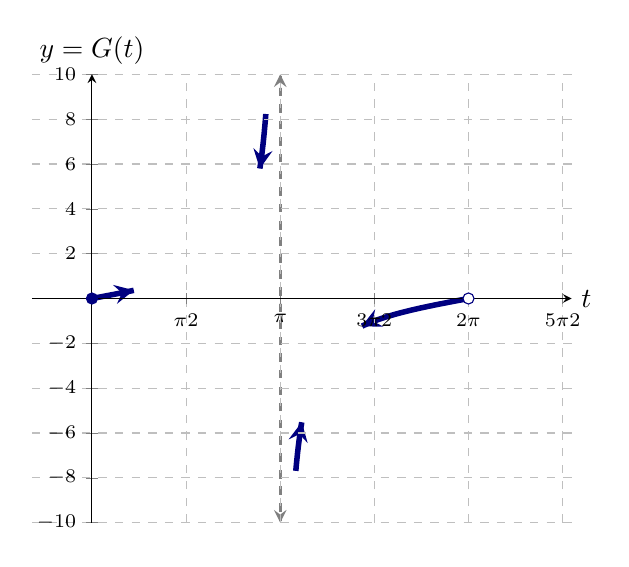
\begin{tikzpicture}
  \begin{axis}[
            domain=-1:8, ymax=10, xmax=8, ymin=-10, xmin=-1,
            axis lines =center, xlabel={$t$}, ylabel={$y = G(t)$}, grid = major, grid style={dashed},
            ytick={-10,-8,-6,-4,-2,2,4,6,8,10},
            xtick={-7.85, -6.28, -4.71, -3.14, -1.57, 0, 1.57, 3.142, 4.71, 6.28, 7.85},
            xticklabels={$\tfrac{-5\pi}{2}$,$-2\pi$,$\tfrac{-3\pi}{2}$,$-\pi$, $\tfrac{-\pi}{2}$, $0$, $\tfrac{\pi}{2}$, $\pi$, $\tfrac{3\pi}{2}$, $2\pi$, $\tfrac{5\pi}{2}$},
            yticklabels={$-10$,$-8$,$-6$,$-4$,$-2$,$2$,$4$,$6$,$8$,$10$}, 
            ticklabel style={font=\scriptsize},
            every axis y label/.style={at=(current axis.above origin),anchor=south},
            every axis x label/.style={at=(current axis.right of origin),anchor=west},
            axis on top
          ]
          

      \addplot [line width=1, gray, dashed,samples=300,domain=(-10:10),<->] ({3.14},{x});

      \addplot[color=penColor,fill=penColor,only marks,mark=*] coordinates{(0,0)};
      \addplot[color=penColor,fill=white,only marks,mark=*] coordinates{(6.28,0)};


            \addplot [line width=2, penColor, smooth,samples=300,domain=(0:0.7),->] {sin(deg(x))/(1 + cos(deg(x)))};
            \addplot [line width=2, penColor, smooth,samples=300,domain=(2.8:2.9),<-] {sin(deg(x))/(1 + cos(deg(x)))};
            \addplot [line width=2, penColor, smooth,samples=300,domain=(3.4:3.5),->] {sin(deg(x))/(1 + cos(deg(x)))};
            \addplot [line width=2, penColor, smooth,samples=300,domain=(4.5:6.28),<-] {sin(deg(x))/(1 + cos(deg(x)))};




  \end{axis}
\end{tikzpicture}
\end{image}






Let's think of the interval $[0, \pi)$ in two pieces  $\left[ 0, \frac{\pi}{2} \right) \cup \left( \frac{\pi}{2}, \pi \right)$.\\


On $\left[ 0, \frac{\pi}{2} \right)$, $\sin(\theta)$ is increasing and $1 + \cos(\theta)$ is decreasing.  This makes the fraction increase.\\


On $\left( \frac{\pi}{2}, \pi \right)$, we know that both the numerator and denominator are approaching $0$.  This makes it difficult to conclude if $G$ is still increasing or not. However, we know that $\lim\limits_{t \to \pi^{-}}G(t) = \infty$ and that is a pretty good signal that $G$ is increasing.



\begin{remark} \textbf{\textcolor{purple!85!blue}{Calculus}}

Calculus will give us a procedure to obtain the derivative of $G$.


\[ G'(t)  = \frac{1}{1 + \cos(t)}    \]



$G'(t)$ is positive, telling us that $G$ is increasing.  Calculus will be tremendously helpful in analyzing functions.

\end{remark}




On the interval $(\pi, 2\pi)$, similar reasoning will tell us that $G$ is increasing. \\


From this we can sketch in a graph.








\begin{image}
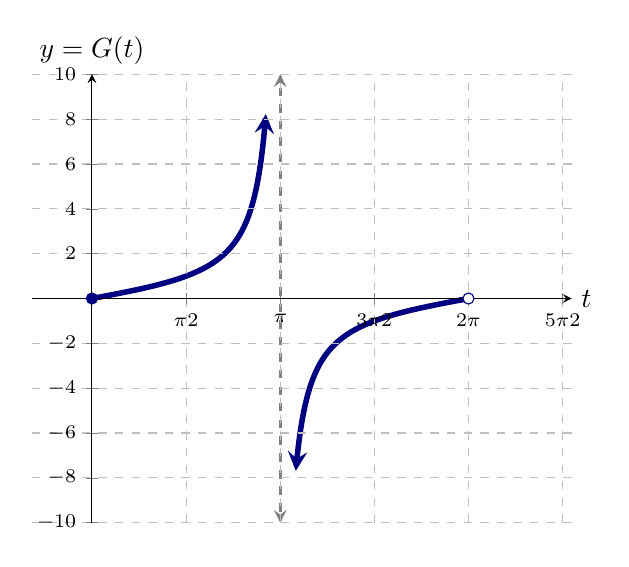
\begin{tikzpicture}
  \begin{axis}[
            domain=-1:8, ymax=10, xmax=8, ymin=-10, xmin=-1,
            axis lines =center, xlabel={$t$}, ylabel={$y = G(t)$}, grid = major, grid style={dashed},
            ytick={-10,-8,-6,-4,-2,2,4,6,8,10},
            xtick={-7.85, -6.28, -4.71, -3.14, -1.57, 0, 1.57, 3.142, 4.71, 6.28, 7.85},
            xticklabels={$\tfrac{-5\pi}{2}$,$-2\pi$,$\tfrac{-3\pi}{2}$,$-\pi$, $\tfrac{-\pi}{2}$, $0$, $\tfrac{\pi}{2}$, $\pi$, $\tfrac{3\pi}{2}$, $2\pi$, $\tfrac{5\pi}{2}$},
            yticklabels={$-10$,$-8$,$-6$,$-4$,$-2$,$2$,$4$,$6$,$8$,$10$}, 
            ticklabel style={font=\scriptsize},
            every axis y label/.style={at=(current axis.above origin),anchor=south},
            every axis x label/.style={at=(current axis.right of origin),anchor=west},
            axis on top
          ]
          

			\addplot [line width=1, gray, dashed,samples=300,domain=(-10:10),<->] ({3.14},{x});

			\addplot[color=penColor,fill=penColor,only marks,mark=*] coordinates{(0,0)};
			\addplot[color=penColor,fill=white,only marks,mark=*] coordinates{(6.28,0)};


            \addplot [line width=2, penColor, smooth,samples=300,domain=(0:2.9),->] {sin(deg(x))/(1 + cos(deg(x)))};
            \addplot [line width=2, penColor, smooth,samples=300,domain=(3.4:6.28),<-] {sin(deg(x))/(1 + cos(deg(x)))};




  \end{axis}
\end{tikzpicture}
\end{image}

And, this is extended periodically. \\



Actually, once we extend this periodically, we might have a better idea. \\









Hmmm, maybe we need a different period to examine.  Let's take a look at $(-\pi, \pi)$.






\begin{image}
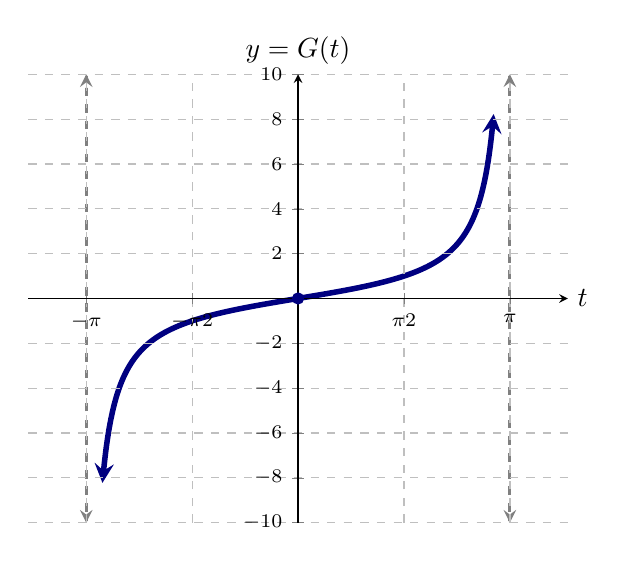
\begin{tikzpicture}
  \begin{axis}[
            domain=-4:4, ymax=10, xmax=4, ymin=-10, xmin=-4,
            axis lines =center, xlabel={$t$}, ylabel={$y = G(t)$}, grid = major, grid style={dashed},
            ytick={-10,-8,-6,-4,-2,2,4,6,8,10},
            xtick={-7.85, -6.28, -4.71, -3.14, -1.57, 0, 1.57, 3.142, 4.71, 6.28, 7.85},
            xticklabels={$\tfrac{-5\pi}{2}$,$-2\pi$,$\tfrac{-3\pi}{2}$,$-\pi$, $\tfrac{-\pi}{2}$, $0$, $\tfrac{\pi}{2}$, $\pi$, $\tfrac{3\pi}{2}$, $2\pi$, $\tfrac{5\pi}{2}$},
            yticklabels={$-10$,$-8$,$-6$,$-4$,$-2$,$2$,$4$,$6$,$8$,$10$}, 
            ticklabel style={font=\scriptsize},
            every axis y label/.style={at=(current axis.above origin),anchor=south},
            every axis x label/.style={at=(current axis.right of origin),anchor=west},
            axis on top
          ]
          

			\addplot [line width=1, gray, dashed,samples=300,domain=(-10:10),<->] ({3.14},{x});
			\addplot [line width=1, gray, dashed,samples=300,domain=(-10:10),<->] ({-3.14},{x});

			\addplot[color=penColor,fill=penColor,only marks,mark=*] coordinates{(0,0)};


            \addplot [line width=2, penColor, smooth,samples=300,domain=(-2.9:2.9),<->] {sin(deg(x))/(1 + cos(deg(x)))};





  \end{axis}
\end{tikzpicture}
\end{image}

That gives a better idea of what is going on.  Remember, this is just one period.




\subsection{Summary}

$\blacktriangleright$ $G$ is a continuous function and has no discontinuities.  

$\blacktriangleright$ All of the odd-$\pi$'s are asymptotic singularities.  The graph has vertical asymptotes.


\begin{itemize}
\item $\lim\limits_{t \to \pi^{-}}G(t) = \infty$ 

\item $\lim\limits_{t \to \pi^{+}}G(t) = -\infty$ 
\end{itemize}


$\blacktriangleright$ This tells us that $G$ has no global maximums or minimums.  

$\blacktriangleright$ Since $G$ is continuous, this also tells us that the range is $(-\infty, \infty)$.  




$\blacktriangleright$ $G$ is an increasing function on any interval in the domain. 


$\blacktriangleright$ $G$ is not an increasing function on its domain. Pick any pair in one interval, there is a ``lower'' pair in the next interval.


$\blacktriangleright$ $G$ is a strictly increasing function on any interval in the domain. 


$\blacktriangleright$ Since $G$ is strictly increasing, there are no local maximums or minimums.









\begin{observation}   \textbf{Tangent?}


The graph kind of looks like a stretched graph of tangent.  Something like $\tan\left( \frac{\theta}{2} \right)$, maybe.






\begin{center}
\desmos{samjrzvval}{400}{300}
\end{center}


Whoa!!!! \\


It appears that


\[   \tan\left( \frac{\theta}{2} \right)   = \frac{\sin(\theta)}{1 + \cos(\theta)}   \]




Or, maybe it looks better like, 




\[   \tan(\theta)   = \frac{\sin(2\theta)}{1 + \cos(2\theta)}   \]





The graph is very suggestive.  Can our algebra verify this? \\


It can.  However, we'll need some more information about sine and cosine.  So, we'll revisit this later.



\end{observation}

















\begin{center}
\textbf{\textcolor{green!50!black}{ooooo-=-=-=-ooOoo-=-=-=-ooooo}} \\

more examples can be found by following this link\\ \link[More Examples of Function Analysis]{https://ximera.osu.edu/csccmathematics/precalculus2/precalculus2/functionAnalysis/examples/exampleList}

\end{center}







\end{document}
